\section{Leaf certificates}\label{sec:leaf}

Suppose that after $t$ rounds \Breaker{} wants to switch to a pairing strategy. He knows the set $B$ of his
own stones. The strategy of \cref{sec:game} does not keep track of all stones of \Maker, however, but
only of a subset $F\subseteq X$, the \emph{revealed} stones, and of their total number $t=|X|$. About the
remaining $\theta=t-|F|$ \emph{unrevealed} stones it knows only that $X$ is \emph{admissible}, a condition
that \Breaker{} enforces by answering immediate threats. A \emph{leaf certificate} is a property of the
triple $(B,F,t)$ which guarantees that there is a pairing for $(B,X)$ for \emph{every} set $X$ that is
compatible with this knowledge. In this section we define admissibility (\cref{ssec:adm}), the certificate
$\CC$ that is needed and the stronger certificate $\LEAF$ that is actually computed (\cref{ssec:certs}); we
show how $\LEAF$ is decided by exact integer computations (\cref{ssec:deciding}), prove that it is monotone
in all its arguments (\cref{ssec:monotone}), and examine the case $F=\emptyset$ (\cref{ssec:Fempty}).

\subsection{Admissible sets}\label{ssec:adm}

\begin{definition}[Threats, danger pairs, admissible sets]\label{def:admissible}
Let $B$ and $X$ be disjoint sets of cells; lines are live or dead with respect to $B$.
\begin{itemize}
\item A \emph{threat} of $X$ is a live line with exactly five cells in $X$.
\item A \emph{danger pair} of $X$ is a pair of distinct live lines $a,b$, each with exactly four cells in
      $X$, that have a common cell which is not in $X$. This cell is the \emph{common cell} of the pair; by
      \cref{lem:geometry}\,\textup{(c)} it is the only common cell of $a$ and $b$.
\item $X$ is \emph{$B$-admissible} if every live line has at most four cells in $X$ and $X$ has no danger
      pair.
\end{itemize}
A set $X$ that meets $B$ is not $B$-admissible.
\end{definition}

The two forbidden configurations are the situations in which \Breaker{} has no time to lose. If \Maker{}
has five stones on a live line, \Breaker{} must take its sixth cell at once. If \Maker's stones form a
danger pair $a,b$ with common cell $c$ and \Maker{} is allowed to play $c$, then $a$ and $b$ become
threats simultaneously and only one of them can be answered; the natural reply of \Breaker{} is to take
$c$ himself, which kills both lines. The strategy of \cref{sec:game} makes exactly these replies, and
\cref{lem:threat,lem:danger} show that after such a reply the stones of \Maker{} are admissible again,
unless \Maker{} has created two such configurations by a single move; this requires at least eleven
stones of \Maker{} (\cref{prop:lost-stones}) and does not happen in the positions that matter. In this
way the admissibility of $X$ is an invariant of the first phase of \Breaker's strategy: it holds at the
beginning of every round until \Breaker{} switches to a pairing (\cref{thm:soundness}).
\Cref{lem:one-two} below shows from another side that admissibility is the right hypothesis: it is precisely Hall's
condition for sets of one and two lines, and hence necessary for the existence of a pairing.

\begin{lemma}[Admissibility is inherited]\label{lem:adm-closed}
Let $B$ and $X$ be disjoint sets of cells.
\begin{enumerate}[label=\textup{(\alph*)}]
\item If $X$ is $B$-admissible and $X'\subseteq X$, then $X'$ is $B$-admissible.
\item If $X$ is $B$-admissible, $B\subseteq B'$ and $B'\cap X=\emptyset$, then $X$ is $B'$-admissible.
\item If a set $F$ is not $B$-admissible, then no set $X\supseteq F$ is $B$-admissible.
\end{enumerate}
\end{lemma}

\begin{proof}
(a) Every live line has at most four cells in $X'$. Suppose that $a,b$ is a danger pair of $X'$ with
common cell $c\notin X'$. Then $|a\cap X|\ge 4$ and $|b\cap X|\ge 4$, so both numbers are $4$, because $X$
is admissible; hence $a\cap X=a\cap X'$ and $b\cap X=b\cap X'$. As $c\in a$ and $c\notin X'$, this gives
$c\notin X$. So $a,b$ is a danger pair of $X$, a contradiction. (b) Every line that is live with respect
to $B'$ is live with respect to $B$, and the two conditions of \cref{def:admissible} concern live lines
only. (c) is the contrapositive of (a).
\end{proof}

\begin{lemma}[Admissibility is Hall's condition for one and two lines]\label{lem:one-two}
Let $B$ and $X$ be disjoint sets of cells. Then $X$ is $B$-admissible if and only if
\begin{enumerate}[label=\textup{(\alph*)}]
\item $|l\setminus X|\ge 2$ for every live line $l$, and
\item $|(a\cup b)\setminus X|\ge 4$ for any two distinct live lines $a,b$.
\end{enumerate}
In particular, if there is a pairing for $(B,X)$, then $X$ is $B$-admissible.
\end{lemma}

\begin{proof}
Condition (a) says that every live line has at most four cells in $X$. Assume that this is the case, and
let $a\ne b$ be live lines. If $a\cap b=\emptyset$, then $|(a\cup b)\setminus X|=|a\setminus X|+|b\setminus
X|\ge 4$. Otherwise $a\cap b=\{c\}$ and $|a\cup b|=11$ by \cref{lem:geometry}\,(c). If $c\in X$, then
$|X\cap(a\cup b)|=|X\cap a|+|X\cap b|-1\le 7$, so $|(a\cup b)\setminus X|\ge 4$. If $c\notin X$, then
$|X\cap(a\cup b)|=|X\cap a|+|X\cap b|\le 8$, with equality if and only if both lines have exactly four
cells in $X$, that is, if and only if $a,b$ is a danger pair; so $|(a\cup b)\setminus X|\ge 4$ fails
exactly for danger pairs. Hence, given (a), condition (b) says that there is no danger pair. The last
statement follows from \cref{lem:hall}\,(b), since (a) and (b) are the instances $|S|=1$ and $|S|=2$ of
Hall's condition.
\end{proof}

\subsection{The certificates \texorpdfstring{$\CC$}{C} and \texorpdfstring{$\LEAF$}{LEAF}}\label{ssec:certs}

\begin{definition}[The certificate $\CC$]\label{def:C}
Let $B,F$ be disjoint sets of cells and $k\ge|F|$ an integer. The statement $\CC(B,F,k)$ is:
\begin{quote}
for every $B$-admissible set $X$ with $F\subseteq X$ and $|X|\le k$ there is a pairing for $(B,X)$.
\end{quote}
The number $\theta=k-|F|$ is the number of unrevealed stones that the certificate allows for.
\end{definition}

This is exactly what \Breaker{} needs at the moment described at the beginning of the section, with
$k=t$. We note some immediate properties.

\begin{remark}\label{rem:C}
(i) If $F$ is not $B$-admissible, $\CC(B,F,k)$ holds vacuously, by \cref{lem:adm-closed}\,(c). Such pairs
$(B,F)$ do not occur in a play in which \Maker's stones are admissible; in \cref{sec:game} the
corresponding states are called \VOID.

(ii) $\CC(B,F,k)$ implies $\CC(B,F',k)$ for $F\subseteq F'$, $|F'|\le k$, and $\CC(B,F,k')$ for
$|F|\le k'\le k$, because the sets $X$ in question form a subfamily. The dependence on $B$ is less
obvious; see \cref{prop:leaf-monotone}\,(c) and \cref{sec:extra-monoC}.

(iii) In terms of the deficiency of \cref{lem:hall}, $\CC(B,F,k)$ says that
\[
  \worst(B,F,k)=\max\{\delta(B,X) : X\ B\text{-admissible},\ F\subseteq X,\ |X|\le k\}
\]
is zero (for $B$-admissible $F$; otherwise the maximum is taken over the empty family). This is the
optimum of an integer program, which is described in \cref{sec:ip} and was used as a cross-check only.

(iv) $\CC(B,F,k)$ can be decided by enumeration. By \cref{lem:adm-closed}\,(a) every $B$-admissible set
$X=F\cup\{c_1,\dots,c_m\}$ with $c_1<\dots<c_m$ is reached by adding the cells $c_1,\dots,c_m$ in this
order through admissible sets; so a depth-first enumeration that adds cells in increasing order and
discards inadmissible sets visits every admissible $X\supseteq F$ with $|X|\le k$, and $\CC(B,F,k)$ holds if
and only if there is a pairing at every set visited. It would not be enough to test the sets with
exactly $k$ cells, since an admissible set need not be contained in an admissible set with $k$ cells. The
enumeration is feasible only for small $\theta$; it serves as a further cross-check in
\cref{sec:verification}.
\end{remark}

Since $\CC$ quantifies over all admissible sets $X$, it is expensive to decide. We replace it by a
stronger condition on $(B,F,k)$ in which $X$ no longer occurs.

\begin{definition}[Surplus, adjacency, connected sets of lines]\label{def:surplus}
Let $B$ be a set of cells, $Y$ a set of cells and $S\subseteq\live{B}$.
\begin{itemize}
\item The \emph{surplus} of $S$ is $\sur_Y(S)=|\N(S)\setminus Y|-2|S|=-\dfc_Y(S)$.
\item Two distinct live lines are \emph{$Y$-adjacent} if they have a common cell that is not in $Y$.
\item $S$ is \emph{$Y$-connected} if $S\ne\emptyset$ and the graph with vertex set $S$ whose edges are
      the $Y$-adjacent pairs is connected. The vertex sets of the connected components of this graph are
      the \emph{$Y$-components} of $S$.
\end{itemize}
\end{definition}

We use these notions for $Y=F$ and, in one proof, for $Y=X$. A set $S$ of live lines with
$\sur_F(S)=\sigma\ge 0$ can absorb $\sigma$ further stones of \Maker{} in $\N(S)$ before Hall's condition
fails for $S$; so one would like every set $S$ to have surplus at least $\theta$. For a single line or
for two lines this is too much to ask (their surplus is at most $4$ and $8$), and it is not needed,
because there admissibility takes over (\cref{lem:one-two}). Sets that are not connected need not be
considered either, because the surplus is additive over components (\cref{lem:additive}). This leads to
the following definition.

\begin{definition}[The certificates $\CPhi$ and $\LEAF$]\label{def:leaf}
Let $B,F$ be disjoint sets of cells. Put
\[
  \Phi(B,F)=\min\{\sur_F(S) : S\subseteq\live{B},\ S\ F\text{-connected},\ |S|\ge 3\},
\]
with $\Phi(B,F)=\infty$ if there is no such $S$. For an integer $k\ge|F|$,
\begin{itemize}
\item $\CPhi(B,F,k)$ is the statement $\Phi(B,F)\ge k-|F|$: every $F$-connected set $S$ of at least three
      live lines has $\sur_F(S)\ge k-|F|$;
\item $\LEAF(B,F,k)$ is the conjunction of
  \begin{enumerate}[label=\textup{(L\arabic*)}]
  \item $F$ is $B$-admissible,
  \item there is a pairing for $(B,F)$,
  \item $\CPhi(B,F,k)$.
  \end{enumerate}
\end{itemize}
\end{definition}

\begin{lemma}[Additivity over components]\label{lem:additive}
Let $Y$ be a set of cells, $S\subseteq\live{B}$, and let $S_1,\dots,S_r$ be the $Y$-components of $S$. Then
the sets $\N(S_i)\setminus Y$ are pairwise disjoint. Consequently
\[
  \sur_Y(S)=\sum_{i=1}^r\sur_Y(S_i)\qquad\text{and}\qquad \dfc_Y(S)=\sum_{i=1}^r\dfc_Y(S_i).
\]
\end{lemma}

\begin{proof}
A cell $c\notin Y$ in $\N(S_i)\cap\N(S_j)$, $i\ne j$, would lie on a line of $S_i$ and on a line of $S_j$;
these two lines would be $Y$-adjacent, which is impossible for lines in different components. Hence
$|\N(S)\setminus Y|=\sum_i|\N(S_i)\setminus Y|$, and $|S|=\sum_i|S_i|$.
\end{proof}

\begin{theorem}[$\LEAF$ implies $\CC$]\label{thm:leaf-implies-C}
Let $B,F$ be disjoint sets of cells and $k\ge|F|$. If $\CPhi(B,F,k)$ holds, then $\CC(B,F,k)$ holds. In
particular, $\LEAF(B,F,k)$ implies $\CC(B,F,k)$.
\end{theorem}

\begin{proof}
Let $X$ be a $B$-admissible set with $F\subseteq X$ and $|X|\le k$, and suppose that there is no pairing for
$(B,X)$. By \cref{lem:hall}\,(b) there is a set $S\subseteq\live{B}$ with $\dfc_X(S)>0$. By
\cref{lem:additive}, applied with $Y=X$, some $X$-component $S'$ of $S$ has $\dfc_X(S')>0$, that is,
\begin{equation}\label{eq:violator}
  |\N(S')\setminus X|<2|S'| ,
\end{equation}
and $S'$ is $X$-connected. We distinguish three cases.

\emph{$|S'|=1$.} Then \eqref{eq:violator} contradicts \cref{lem:one-two}\,(a).

\emph{$|S'|=2$.} Then \eqref{eq:violator} contradicts \cref{lem:one-two}\,(b).

\emph{$|S'|\ge 3$.} Since $F\subseteq X$, a common cell of two lines that is not in $X$ is not in $F$; so
$X$-adjacent lines are $F$-adjacent, and $S'$ is $F$-connected. By $\CPhi(B,F,k)$,
\[
  |\N(S')\setminus F|-2|S'|\ \ge\ k-|F|\ \ge\ |X|-|F|\ =\ |X\setminus F|\ \ge\ |(X\setminus F)\cap\N(S')| .
\]
Hence $|\N(S')\setminus X|=|\N(S')\setminus F|-|(X\setminus F)\cap\N(S')|\ge 2|S'|$, contradicting
\eqref{eq:violator}.
\end{proof}

\begin{remark}\label{rem:leaf}
(i) The proof uses only condition (L3). If (L1) fails, $\CC(B,F,k)$ is vacuous (\cref{rem:C}\,(i)).

(ii) Conditions (L1) and (L3) imply (L2): by the theorem $\CC(B,F,k)$ holds, and $X=F$ is a $B$-admissible
set with $|X|\le k$. We keep (L2) in the definition because the algorithm that decides (L3) starts from a
pairing for $(B,F)$; the three conditions are evaluated in this order (\cref{alg:leaf}).

(iii) For $\theta=0$ the certificate is exact. Indeed, $\CPhi(B,F,|F|)$ says that $\sur_F(S)\ge 0$ for
certain sets $S$, which follows from (L2) by \cref{lem:hall}\,(b). So $\LEAF(B,F,|F|)$ holds if and only if
$F$ is $B$-admissible and there is a pairing for $(B,F)$; for $B$-admissible $F$ this is precisely
$\CC(B,F,|F|)$, in which $X=F$ is the only set to be considered.

(iv) In general $\LEAF$ is only sufficient for $\CC$: a set $S$ with small surplus is harmless if the
cells of $\N(S)$ cannot take $\theta$ further stones in an admissible way. \Cref{ex:C-not-leaf} gives an
instance that can be checked by hand; instances with $F\ne\emptyset$ that are closer to positions of the
game were found in the cross-checks of \cref{sec:verification}. The two certificates agree for $\theta=0$
by (iii), and for $F=\emptyset$ and $k\le 10$ by \cref{prop:leaf-equals-C}.
\end{remark}

\begin{example}[$\CC$ holds, $\LEAF$ fails]\label{ex:C-not-leaf}
Let $o=(0,0,0)$, and let $T$ consist of the three lines through $o$ in the plane $x=0$,
\[
  a_1=\{(0,0,t)\},\qquad a_2=\{(0,t,0)\},\qquad a_3=\{(0,t,t)\}\qquad(0\le t\le 5),
\]
so that $|\N(T)|=3\cdot 5+1=16$. Let $B=\Q\setminus\N(T)$, a set of $200$ cells, $F=\emptyset$ and $k=11$.
(This is an instance of the predicates, not a position of the game.)

\emph{$\LEAF(B,\emptyset,11)$ is false.} A line $l\notin T$ meets each line of $T$ in at most one cell, so
it has at most three cells in $\N(T)$ and contains a cell of $B$. Hence $\live{B}=T$. The set $T$ is
$\emptyset$-connected, since its lines have the common cell $o$, and $\sur_\emptyset(T)=16-6=10<11$. So
(L3) fails.

\emph{$\CC(B,\emptyset,11)$ is true.} Let $X$ be $B$-admissible; then $X\subseteq\N(T)$. We claim that
$|X|\le 10$. If $o\in X$, the three numbers $|X\cap a_i|$ are at most $4$ and add up to $|X|+2$. If
$o\notin X$, at most one line of $T$ has four cells in $X$, since two such lines would be a danger pair
with common cell $o$; so $|X|\le 4+3+3$. Now we verify Hall's condition for the non-empty subsets $S$ of
$\live{B}=T$. For $|S|=1$ and $|S|=2$ it holds by \cref{lem:one-two}. For $S=T$ we have
$|\N(T)\setminus X|\ge 16-10=6=2|T|$. By \cref{lem:hall}\,(b) there is a pairing for $(B,X)$.
\end{example}

\subsection{Deciding \texorpdfstring{$\LEAF$}{LEAF}: triples and augmenting paths}\label{ssec:deciding}

Conditions (L1) and (L2) are decided directly from the definitions, (L2) by bipartite matching
(\cref{lem:hall}). Condition (L3) quantifies over all $F$-connected sets of live lines, of which there
may be exponentially many. We show that it suffices to consider the $F$-connected sets of three lines,
and that for each of them the relevant minimum of the surplus is obtained by augmenting a pairing. The
results of this subsection justify the algorithm of \cref{sec:verification} (\cref{alg:leaf}); they are
not needed for the implication $\LEAF\Rightarrow\CC$.

Throughout this subsection $B$ and $F$ are fixed disjoint sets of cells, and $\theta\ge 0$ is an integer.
An \emph{$F$-connected triple} is an $F$-connected set of three live lines. For a set $U\subseteq\live{B}$
let
\[
  \mu(U)=\min\{\sur_F(S) : U\subseteq S\subseteq\live{B}\}.
\]

\begin{lemma}\label{lem:triple}
Every $F$-connected set $S$ of at least three live lines contains an $F$-connected triple.
\end{lemma}

\begin{proof}
A spanning tree of the graph of $F$-adjacency on $S$ has at least three vertices and therefore a vertex
of degree at least $2$ (a tree in which all degrees are at most $1$ has at most one edge). This vertex
and two of its neighbors form an $F$-connected triple.
\end{proof}

\begin{proposition}[Reduction to triples]\label{prop:triples}
Assume that there is a pairing for $(B,F)$.
\begin{enumerate}[label=\textup{(\alph*)}]
\item For every $F$-connected set $U\subseteq\live{B}$ the minimum defining $\mu(U)$ is attained by an
      $F$-connected set:
      \[ \mu(U)=\min\{\sur_F(S) : U\subseteq S\subseteq\live{B},\ S\ F\text{-connected}\}. \]
\item $\Phi(B,F)=\min\{\mu(T) : T \text{ an $F$-connected triple}\}$. Hence $\CPhi(B,F,k)$ holds if and only
      if $\mu(T)\ge k-|F|$ for every $F$-connected triple $T$.
\end{enumerate}
The inequality $\Phi(B,F)\ge\min_T\mu(T)$, and with it the implication ``if'' in \textup{(b)}, holds also
without the assumption.
\end{proposition}

\begin{proof}
(a) The inequality ``$\le$'' is trivial. Let $S\supseteq U$ be an arbitrary subset of $\live{B}$, and let
$S_0$ be the $F$-component of $S$ that contains $U$; it exists because $U$ is $F$-connected. By
\cref{lem:additive}, $\sur_F(S)$ is the sum of $\sur_F(S_0)$ and of the surpluses of the other
$F$-components of $S$, each of which is non-negative by \cref{lem:hall}\,(b), because there is a pairing
for $(B,F)$. Hence $\sur_F(S)\ge\sur_F(S_0)$, where $S_0\supseteq U$ is $F$-connected.

(b) An $F$-connected set $S$ with $|S|\ge 3$ contains an $F$-connected triple $T$ (\cref{lem:triple}), and
$\sur_F(S)\ge\mu(T)$ by the definition of $\mu$; this shows $\Phi(B,F)\ge\min_T\mu(T)$ and does not use the
pairing. Conversely, for an $F$-connected triple $T$ there is by (a) an $F$-connected set $S_0\supseteq T$
with $\sur_F(S_0)=\mu(T)$; as $|S_0|\ge 3$, we get $\Phi(B,F)\le\mu(T)$.
\end{proof}

To compute $\mu(U)$ we let the lines of $U$ collect as many cells as possible, while every other live
line keeps two.

\begin{definition}[$U$-assignments and augmenting paths]\label{def:U-assignment}
Let $U\subseteq\live{B}$.
\begin{itemize}
\item A \emph{$U$-assignment} is a map $\alpha$ from a set $\operatorname{dom}(\alpha)$ of cells to
      $\live{B}$ such that $c\in\alpha(c)$ and $c\notin F$ for every $c\in\operatorname{dom}(\alpha)$, every
      line of $\live{B}\setminus U$ is the image of exactly two cells, and every line of $U$ is the image
      of at least two cells. The cells of $\operatorname{dom}(\alpha)$ are \emph{assigned}; the line $l$
      \emph{holds} the cells of $\alpha^{-1}(l)\subseteq l\setminus F$. The \emph{excess} of $\alpha$ is
      \[
        e(\alpha)=|\operatorname{dom}(\alpha)|-2|\live{B}|=\sum_{l\in U}\bigl(|\alpha^{-1}(l)|-2\bigr).
      \]
\item An \emph{alternating path} from a line $l_0$ (with respect to $\alpha$) is a sequence
      \[ l_0,\,c_1,\,l_1,\,\dots,\,c_j,\,l_j\qquad(j\ge 0) \]
      of distinct live lines $l_i$ and of cells $c_i$ such that
      $c_i\in l_{i-1}\setminus F$ and $\alpha(c_i)=l_i$ for $1\le i\le j$. A line is \emph{reachable} from
      $l_0$ if it is the last line of an alternating path from $l_0$; for a set $U'$ of lines,
      $R_\alpha(U')$ denotes the set of lines that are reachable from some line of $U'$. In particular
      $U'\subseteq R_\alpha(U')$.
\item An \emph{augmenting path} from $l_0$ is an alternating path $l_0,c_1,\dots,l_j$ from $l_0$ together
      with a cell $c_{j+1}\in l_j\setminus F$ that is not assigned. To \emph{augment} $\alpha$ along it
      means to replace $\alpha$ by the map $\alpha'$ with $\alpha'(c_i)=l_{i-1}$ for $1\le i\le j+1$ and
      $\alpha'(c)=\alpha(c)$ for all other $c\in\operatorname{dom}(\alpha)$.
\item A set $R\subseteq\live{B}$ is \emph{closed} (with respect to $\alpha$) if every cell of
      $\N(R)\setminus F$ is held by a line of $R$.
\end{itemize}
\end{definition}

A pairing $\pi$ for $(B,F)$, regarded as the map that sends the two cells of $\pi(l)$ to $l$, is a
$U$-assignment of excess $0$ for every $U$. We record three simple facts about these notions.
\begin{enumerate}[label=\textup{(\roman*)}]
\item In an alternating path the cell $c_i$ is held by $l_i\ne l_{i-1}$, so it is not held by $l_{i-1}$;
      and the cells $c_1,\dots,c_j$ are distinct, because they are held by distinct lines.
\item If $\alpha$ is a $U$-assignment and $l_0\in U$, augmenting along an augmenting path from $l_0$ gives a
      $U$-assignment $\alpha'$ with $e(\alpha')=e(\alpha)+1$. Indeed, the line $l_0$ gains the cell $c_1$;
      each line $l_i$, $1\le i\le j$, loses $c_i$ and gains $c_{i+1}$, which it did not hold; no other line
      is affected; and exactly one new cell, $c_{j+1}$, is assigned.
\item If a line $l$ is reachable from $l_0$, and a cell $c\in l\setminus F$ is held by a line $l'\ne l$,
      then $l'$ is reachable from $l_0$: either $l'$ already occurs on an alternating path from $l_0$ to
      $l$, or this path can be extended by $c,l'$.
\end{enumerate}

\begin{proposition}[Computing $\mu$ by augmentation]\label{prop:maxflow}
Let $\pi$ be a pairing for $(B,F)$ and $U\subseteq\live{B}$.
\begin{enumerate}[label=\textup{(\alph*)}]
\item \textup{(Upper bound.)} For every $U$-assignment $\alpha$ and every set $S$ with
      $U\subseteq S\subseteq\live{B}$ we have $e(\alpha)\le\sur_F(S)$. Hence $e(\alpha)\le\mu(U)$.
\item \textup{(Closed sets persist.)} Let $R$ be closed with respect to a $U$-assignment $\alpha$. Then no
      augmenting path contains a line of $R$. Augmenting $\alpha$ along any augmenting path changes
      $\alpha(c)$ for no cell $c\in\N(R)\setminus F$, and $R$ is closed with respect to the new assignment.
\item \textup{(Witness.)} Let $\alpha$ be a $U$-assignment and $U'\subseteq U$ a set such that there is no
      augmenting path from any line of $U'$. Then $R=R_\alpha(U')$ is closed. If $U'=U$, then moreover
      \[
        \sur_F(R)=e(\alpha)=\mu(U),
      \]
      and $R$ is $F$-connected if $U$ is.
\item \textup{(Augmentation.)} Start with $\alpha=\pi$ and augment repeatedly along augmenting paths from
      lines of $U$, chosen arbitrarily, until there is no such path. Then exactly $\mu(U)$ augmentations
      are performed. In particular, $\mu(U)\ge\theta$ if and only if $\theta$ successive augmentations
      are possible.
\item \textup{(One line at a time.)} Let $U=\{u_1,\dots,u_m\}$. Start with $\alpha=\pi$; augment along
      augmenting paths from $u_1$ until there is none, then along augmenting paths from $u_2$ until there
      is none, and so on. After the step for $u_m$ there is no augmenting path from any line of $U$, so
      that again exactly $\mu(U)$ augmentations have been performed.
\end{enumerate}
\end{proposition}

\begin{proof}
(a) The cells held by the lines of $S$ are distinct cells of $\N(S)\setminus F$. Their number is
$\sum_{l\in S}|\alpha^{-1}(l)|=2|S|+e(\alpha)$, because $U\subseteq S$ and every line outside $U$ holds exactly
two cells. Hence $2|S|+e(\alpha)\le|\N(S)\setminus F|$.

(b) Let $l_0,c_1,\dots,l_j,c_{j+1}$ be an augmenting path and suppose that $l_i\in R$ for some $i\le j$. The
cell $c_{i+1}\in l_i\setminus F$ lies in $\N(R)\setminus F$, so it is held by a line of $R$. In particular
it is assigned, hence $i<j$, and $l_{i+1}=\alpha(c_{i+1})\in R$. Repeating the argument we arrive at
$l_j\in R$ and conclude that $c_{j+1}$ is assigned, a contradiction. Thus no augmenting path contains a
line of $R$. Augmenting changes the value of $\alpha$ only at the cells $c_1,\dots,c_{j+1}$ of the path. If
one of them, say $c_i$, belonged to $\N(R)\setminus F$, it would be held by a line of $R$; then $i\le j$
and $l_i=\alpha(c_i)\in R$, which we have just excluded. So the cells of $\N(R)\setminus F$ keep their
lines, and $R$ remains closed.

(c) Let $l\in R$ and $c\in l\setminus F$. If $c$ were not assigned, an alternating path from a line of
$U'$ to $l$ together with $c$ would be an augmenting path from a line of $U'$. So $c$ is held by a line
$l'$, and $l'=l$ or $l'$ is reachable by fact~(iii) above; in both cases $l'\in R$. Hence $R$ is closed.
Now let $U'=U$, so that $U\subseteq R$. The lines of $R$ hold cells of $\N(R)\setminus F$ only, and every
cell of $\N(R)\setminus F$ is held by a line of $R$; therefore
\[
  |\N(R)\setminus F|=\sum_{l\in R}|\alpha^{-1}(l)|=2|R|+e(\alpha),
\]
again because $U\subseteq R$ and the lines outside $U$ hold exactly two cells. Thus $\sur_F(R)=e(\alpha)$,
and by (a) we get $e(\alpha)\le\mu(U)\le\sur_F(R)=e(\alpha)$. Finally, consecutive lines $l_{i-1},l_i$ of an
alternating path are $F$-adjacent, since they share the cell $c_i\notin F$, and all lines of an
alternating path from a line of $U$ belong to $R$. So every line of $R$ is joined to a line of $U$ by a
path of $F$-adjacent lines inside $R$, and $R$ is $F$-connected if $U$ is.

(d) By fact~(ii) every augmentation yields a $U$-assignment and raises the excess by $1$; by (a) the
excess never exceeds $\mu(U)$, which is finite (take $S=\live{B}$), so the procedure stops. When it stops,
there is no augmenting path from any line of $U$, and $e(\alpha)=\mu(U)$ by (c) with $U'=U$. Since the
excess of $\pi$ is $0$, exactly $\mu(U)$ augmentations were performed. If $\mu(U)\ge\theta$, the procedure
therefore does not stop before the $\theta$-th augmentation; conversely, after $\theta$ augmentations
the excess is $\theta\le\mu(U)$ by (a).

(e) When the step for $u_i$ ends, there is no augmenting path from $u_i$, so $R_i=R_\alpha(\{u_i\})$ is
closed by (c), applied with $U'=\{u_i\}$, and $u_i\in R_i$. By (b), $R_i$ stays closed during all later
augmentations, and as long as $R_i$ is closed there is no augmenting path from $u_i\in R_i$. Hence at the
end there is no augmenting path from any line of $U$, and the number of augmentations is $\mu(U)$ by (d).
\end{proof}

\begin{remark}[Flows]\label{rem:flow}
In the language of flows, let $\mathcal N_U$ be the network $\mathcal N(B,F)$ of \cref{lem:hall}\,(c) in
which the arcs $s\to l$ with $l\in U$ have unbounded capacity. A $U$-assignment is an integral flow in
$\mathcal N_U$ that saturates the arcs $s\to l$ for $l\notin U$ and sends at least two units through
each arc $s\to l$ with $l\in U$; its value is $2|\live{B}|+e(\alpha)$. The
augmenting paths of \cref{def:U-assignment} are the augmenting paths from $s$ to $t$ in the residual
network (they start with an arc $s\to l_0$, $l_0\in U$, since the other arcs out of $s$ are saturated),
and $R_\alpha(U)$ is the set of lines that can be reached from $s$ in the residual network. Thus
\cref{prop:maxflow} says that the maximum flow value of $\mathcal N_U$ is $2|\live{B}|+\mu(U)$, and that
a maximum flow is reached from $\pi$ by exactly $\mu(U)$ augmentations; this also follows from the
max-flow min-cut theorem~\cite{FordFulkerson1962} by the computation in the proof of \cref{lem:hall}.

One point requires care in an implementation that uses a finite capacity on the arcs $s\to l$, $l\in U$.
At most $|l\setminus F|\le 6$ units can pass through a line $l$, so any capacity of at least $6$ gives
the same maximum flow. But with capacity exactly $6$ such an arc is saturated when $l$ holds all its six
cells, and $l$ is then not reachable from $s$ in the residual network: for $U=\{l\}$, $F\cap
l=\emptyset$ and an assignment in which $l$ holds its six cells, no line is reachable from $s$, although
the witness of \cref{prop:maxflow}\,(c) is $R_\alpha(U)\ni l$. To obtain the witness one must either use a
capacity of at least $7$, or add the lines of $U$ to the reachable set explicitly, as
\cref{def:U-assignment} does.
\end{remark}

\begin{corollary}[Pruning rules and quick rejection]\label{cor:pruning}
Let $\pi$ be a pairing for $(B,F)$.
\begin{enumerate}[label=\textup{(\alph*)}]
\item If $U\subseteq U'\subseteq\live{B}$, then $\mu(U)\le\mu(U')$. Hence, for an $F$-connected triple $T$:
      if $\mu(\{l\})\ge\theta$ for one line $l\in T$, or $\mu(\{a,b\})\ge\theta$ for two lines $a,b\in T$,
      then $\mu(T)\ge\theta$.
\item Let $S$ be an $F$-component of the set $\live{B}$ of all live lines. Then the number of cells of
      $\N(S)\setminus F$ that are not assigned by $\pi$ is equal to $\sur_F(S)$. Hence, if $|S|\ge 3$ and
      $\pi$ leaves fewer than $\theta$ cells of $\N(S)\setminus F$ unassigned, then
      $\Phi(B,F)\le\sur_F(S)<\theta$.
\end{enumerate}
\end{corollary}

\begin{proof}
(a) The minimum defining $\mu(U')$ is taken over a subfamily of the sets admitted for $\mu(U)$. (b) Let
$c\in\N(S)\setminus F$ be assigned to a line $l'$, and let $l\in S$ be a line through $c$. If $l'\ne l$,
then $l'$ and $l$ are $F$-adjacent, so $l'\in S$, because $S$ is a component of the whole set $\live{B}$.
Thus every assigned cell of $\N(S)\setminus F$ is held by a line of $S$. Conversely, the $2|S|$ cells held
by the lines of $S$ lie in $\N(S)\setminus F$. So exactly $2|S|$ cells of $\N(S)\setminus F$ are assigned,
and $|\N(S)\setminus F|-2|S|=\sur_F(S)$ are not.
\end{proof}

Since a single line holds at most six cells and two lines at most twelve, we have $\mu(\{l\})\le 4$ and
$\mu(\{a,b\})\le 8$; so the first rule in (a) can apply only for $\theta\le 4$ and the second only for
$\theta\le 8$. In (b), counting the cells of $F\cap\N(S)$ as unassigned as well makes the test weaker but
leaves it valid.

\medskip\noindent\textbf{An exact test for $\LEAF$.}
Together these results give the following procedure for deciding $\LEAF(B,F,k)$, where
$\theta=k-|F|\ge 0$. All its steps are computations with small integers on a bipartite graph with at
most $148+216$ vertices.
\begin{enumerate}[label=\textup{\arabic*.}]
\item Test whether $F$ is $B$-admissible (\cref{def:admissible}). If not, $\LEAF(B,F,k)$ is false.
\item Compute a maximum assignment for $(B,F)$ by augmenting paths (\cref{lem:hall}). If some live line
      receives fewer than two cells, there is no pairing and $\LEAF(B,F,k)$ is false. Otherwise a pairing
      $\pi$ has been found.
\item Optionally, apply the quick rejection of \cref{cor:pruning}\,(b) to the $F$-components of
      $\live{B}$ with at least three lines.
\item For every $F$-connected triple $T$ (a line together with two lines that are $F$-adjacent to it),
      decide whether $\mu(T)\ge\theta$: starting from $\pi$, try to perform $\theta$ augmentations from
      the lines of $T$ (\cref{prop:maxflow}\,(d) or (e)). A triple may be skipped if one of its lines or
      pairs of lines is already known to satisfy $\mu\ge\theta$ (\cref{cor:pruning}\,(a)). If the
      procedure stops after fewer than $\theta$ augmentations, then $R=R_\alpha(T)$ is an $F$-connected
      set of at least three live lines with $\sur_F(R)=\mu(T)<\theta$ (\cref{prop:maxflow}\,(c)), and
      $\LEAF(B,F,k)$ is false.
\item If every triple passes, $\LEAF(B,F,k)$ is true (\cref{prop:triples}\,(b)).
\end{enumerate}
A negative answer in steps 3 and 4 comes with a set $S$ of lines whose surplus can be recomputed from
the definition, and a positive answer for a triple $T$ comes with a $T$-assignment of excess $\theta$,
which by \cref{prop:maxflow}\,(a) proves $\sur_F(S)\ge\theta$ for all $S\supseteq T$ without any reference
to the way in which it was found. For the soundness of the main theorem only positive answers matter,
and for these the argument just given, \cref{lem:triple} and \cref{thm:leaf-implies-C} suffice.

\subsection{Monotonicity}\label{ssec:monotone}

The certificate $\LEAF$ can only improve when more stones of \Maker{} are revealed, when fewer stones
have to be allowed for, and when \Breaker{} has more stones.

\begin{proposition}[Monotonicity of $\LEAF$]\label{prop:leaf-monotone}
Assume that $\LEAF(B,F,k)$ holds.
\begin{enumerate}[label=\textup{(\alph*)}]
\item If $F\subseteq F'$, $F'$ is $B$-admissible and $|F'|\le k$, then $\LEAF(B,F',k)$ holds.
\item If $|F|\le k'\le k$, then $\LEAF(B,F,k')$ holds.
\item If $b$ is a cell with $b\notin F$, then $\LEAF(B+b,F,k)$ holds.
\end{enumerate}
\end{proposition}

\begin{proof}
(a) (L1) is assumed. (L2): by \cref{thm:leaf-implies-C}, $\CC(B,F,k)$ holds, and $F'$ is a $B$-admissible
set with $F\subseteq F'$ and $|F'|\le k$; so there is a pairing for $(B,F')$. (L3): let $S$ be an
$F'$-connected set of at least three live lines. A common cell of two lines outside $F'$ is outside
$F$, so $S$ is $F$-connected, and
\[
  \sur_{F'}(S)=\sur_F(S)-|\N(S)\cap(F'\setminus F)|\ \ge\ (k-|F|)-|F'\setminus F|=k-|F'| .
\]

(b) (L1) and (L2) do not involve $k$, and $k'-|F|\le k-|F|$.

(c) (L1) holds by \cref{lem:adm-closed}\,(b), since $(B+b)\cap F=\emptyset$. (L2) holds by
\cref{lem:hall}\,(e). (L3): a set of lines that are live with respect to $B+b$ is a set of lines that are
live with respect to $B$, and neither $F$-adjacency nor $\sur_F$ depends on $B$.
\end{proof}

In terms of \cref{def:leaf}, (a) says that $\Phi(B,F')\ge\Phi(B,F)-|F'\setminus F|$ and (c) says that
$\Phi(B+b,F)\ge\Phi(B,F)$. These properties make $\LEAF$ well suited to a search for certificates; within
this paper, (a) is used in the proof of \cref{prop:lazy-monotone}, and \cref{thm:soundness} does not
depend on the proposition. For the certificate $\CC$ the analogue of (c) is true only for $B$-admissible
$F$, and its proof is considerably longer; it is given in \cref{sec:extra-monoC} and is not used
anywhere.

\subsection{The case \texorpdfstring{$F=\emptyset$}{F empty}}\label{ssec:Fempty}

For $F=\emptyset$ two lines are adjacent if they meet, and we write $\sur(S)$ for $\sur_\emptyset(S)$ and
``connected'' for ``$\emptyset$-connected''. By \cref{lem:geometry}\,(c) a connected set $T$ of three
lines is of one of three kinds:
\begin{itemize}
\item a \emph{triangle}: the three lines meet pairwise, in three distinct cells; $|\N(T)|=18-3=15$ and
      $\sur(T)=9$;
\item a \emph{star}: the three lines pass through one cell; $|\N(T)|=16$ and $\sur(T)=10$;
\item a \emph{path}: two of the lines are disjoint and the third meets both; $|\N(T)|=16$ and
      $\sur(T)=10$.
\end{itemize}
(If the three lines meet pairwise and two of the three meeting cells coincide, this cell lies on all
three lines, and all three meeting cells coincide.)

\begin{lemma}[Ten admissible stones on three lines]\label{lem:433}
Let $a_1,a_2,a_3$ be three distinct live lines, and call a cell of $a_i$ \emph{private} if it lies on
neither of the other two lines. Then each $a_i$ has at least four private cells. If $X_T$ consists of
four private cells of $a_1$, three private cells of $a_2$ and three private cells of $a_3$, then
$|X_T|=10$, and $X_T$ and all its subsets are $B$-admissible.
\end{lemma}

\begin{proof}
Each $a_i$ meets each of the other two lines in at most one cell, so at least four of its cells are
private. A private cell of $a_j$ does not lie on $a_i$ for $i\ne j$; hence the ten chosen cells are
distinct, and $a_1,a_2,a_3$ contain exactly $4$, $3$, $3$ cells of $X_T$. Any other line meets each $a_i$
in at most one cell and so contains at most three cells of $X_T$. Thus no line has more than four cells
in $X_T$, and only one line has four, so there is no danger pair. Moreover $X_T\cap B=\emptyset$, because
the lines are live. The subsets of $X_T$ are $B$-admissible by \cref{lem:adm-closed}\,(a).
\end{proof}

\begin{proposition}[$\LEAF$ is exact for $F=\emptyset$, $k\le 10$]\label{prop:leaf-equals-C}
For every set $B$ of cells and every integer $k$ with $0\le k\le 10$,
\[
  \CC(B,\emptyset,k)\iff\LEAF(B,\emptyset,k).
\]
\end{proposition}

\begin{proof}
``$\Leftarrow$'' is \cref{thm:leaf-implies-C}. For ``$\Rightarrow$'' assume $\CC(B,\emptyset,k)$. Condition
(L1) is trivial, and (L2) is $\CC(B,\emptyset,k)$ applied to $X=\emptyset$. Suppose that (L3) fails: there is
a connected set $S\subseteq\live{B}$ with $|S|\ge 3$ and $\sur(S)\le k-1\le 9$. By (L2) and
\cref{lem:hall}\,(b), $\sur(S)\ge 0$. Put $j=\sur(S)+1$, so that $1\le j\le k\le 10$. Choose a connected
triple $T\subseteq S$ (\cref{lem:triple}) and a subset $X$ with $j$ elements of a set $X_T$ as in
\cref{lem:433}. Then $X$ is $B$-admissible, $|X|=j\le k$, and $X\subseteq\N(T)\subseteq\N(S)$, so that
\[
  |\N(S)\setminus X|=|\N(S)|-j=2|S|+\sur(S)-j=2|S|-1<2|S| .
\]
By \cref{lem:hall}\,(b) there is no pairing for $(B,X)$, which contradicts $\CC(B,\emptyset,k)$.
\end{proof}

The bound $10$ is the size of $X_T$. For $k\ge 11$, or for $F\ne\emptyset$, the construction is not
available, and $\LEAF$ is only sufficient for $\CC$ (\cref{ex:C-not-leaf}).

\begin{corollary}[Slack is necessary]\label{cor:slack-necessary}
Let $B$ be a set of cells with at least three live lines and let $k\le 10$. If $\LEAF(B,\emptyset,k)$
holds, then $\slack(B)\ge k$.
\end{corollary}

\begin{proof}
Choose three live lines and a subset $X$ with $k$ elements of a set $X_T$ as in \cref{lem:433}. By
\cref{thm:leaf-implies-C} there is a pairing for $(B,X)$, and $k=|X|\le\slack(B)$ by
\cref{lem:slack-bound}.
\end{proof}

For $F=\emptyset$ a triangle of live lines limits the certificate to $k\le 9$, since its surplus is $9$.
Sets of busy cells cannot destroy all triangles unless they are large:

\begin{proposition}[Busy sets with at most eleven cells]\label{prop:busy10}
Let $B\subseteq\Busy$ be a set of busy cells with $|B|\le 11$. Then $\live{B}$ contains a triangle.
Consequently $\Phi(B,\emptyset)\le 9$, and $\LEAF(B,\emptyset,k)$ and $\CC(B,\emptyset,k)$ are false for
every $k\ge 10$. In particular, $\LEAF(B,\emptyset,10)$ is false for every set $B$ of ten busy cells.
\end{proposition}

\begin{proof}
A busy cell lies on exactly three face diagonals (\cref{lem:degree}). So at most $33$ of the $36$ face
diagonals contain a cell of $B$, and there is a live face diagonal $d$. A permutation of the coordinates
maps lines onto lines and busy cells onto busy cells (\cref{lem:group}); we may therefore assume that the
constant coordinate of $d$ is the third one, with value $v$, so that
\[
  d=\{(t,t,v):0\le t\le 5\}\qquad\text{or}\qquad d=\{(t,5-t,v):0\le t\le 5\}.
\]
There are four values in $\{0,\dots,5\}$ whose level is different from $\lambda(v)$, and they form two
pairs $\{i,5-i\}$. Let $r$ be a value from one of these pairs and $s$ a value from the other; thus
$\lambda(r)\ne\lambda(v)$, $\lambda(s)\ne\lambda(v)$, and $s\notin\{r,5-r\}$. Consider the axis lines
\[
  a=\{(t,r,v):0\le t\le 5\}\qquad\text{and}\qquad b=\{(s,t,v):0\le t\le 5\}.
\]
By \cref{lem:busy}\,(b) neither of them contains a busy cell, since their constant coordinates have
different levels. Hence $a$ and $b$ are live, like $d$. We have $a\cap b=\{(s,r,v)\}$, and
\[
  d\cap a=\{(r,r,v)\},\quad d\cap b=\{(s,s,v)\}\qquad\text{or}\qquad
  d\cap a=\{(5-r,r,v)\},\quad d\cap b=\{(s,5-s,v)\}
\]
in the two cases. Since $s\ne r$ and $s\ne 5-r$, the three meeting cells are distinct in both cases. So
$T=\{d,a,b\}$ is a triangle of live lines.

Now $T$ is a connected set of three live lines with $\sur(T)=15-6=9$; hence $\Phi(B,\emptyset)\le 9$, and
$\LEAF(B,\emptyset,k)$ is false for $k\ge 10$. By \cref{prop:leaf-equals-C}, $\CC(B,\emptyset,10)$ is false,
and so is $\CC(B,\emptyset,k)$ for every $k\ge 10$ by \cref{rem:C}\,(ii).
\end{proof}

\begin{figure}[t]
\centering
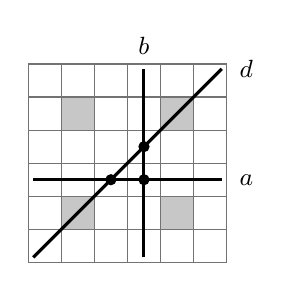
\begin{tikzpicture}[scale=0.42]
\foreach \x in {1,4} { \foreach \y in {1,4} { \fill[black!22] (\x,\y) rectangle ++(1,1); } }
\draw[step=1,black!55,thin] (0,0) grid (6,6);
\draw[line width=1.1pt] (0.15,0.15) -- (5.85,5.85);
\draw[line width=1.1pt] (0.15,2.5) -- (5.85,2.5);
\draw[line width=1.1pt] (3.5,0.15) -- (3.5,5.85);
\fill (2.5,2.5) circle (0.17); \fill (3.5,3.5) circle (0.17); \fill (3.5,2.5) circle (0.17);
\node[right] at (6.1,5.85) {\small $d$};
\node[right] at (6.1,2.5) {\small $a$};
\node[above] at (3.5,6.0) {\small $b$};
\end{tikzpicture}
\caption{The triangle in the proof of \cref{prop:busy10}, drawn in the plane $z=v$ for $v=1$, with
$d=\{(t,t,1)\}$, $r=2$ and $s=3$ ($x$ to the right, $y$ upwards). Shaded: the four busy cells of the
plane. The lines $a$ (row $y=r$) and $b$ (column $x=s$) contain no busy cell.}
\label{fig:triangle}
\end{figure}

More generally, if $T$ is a triangle of live lines none of whose three meeting cells belongs to $F$,
then $T$ is $F$-connected and $\Phi(B,F)\le\sur_F(T)=9-|F\cap\N(T)|$. In the certificate of
\cref{sec:certificate} the largest number of unrevealed stones at a leaf is $\theta=8$.

We finally return to the examples of \cref{ssec:examples}.

\begin{fact}[The sets $\Teight$ and $\Tseven$]\label{fact:T8-leaf}
\begin{enumerate}[label=\textup{(\alph*)}]
\item $\LEAF(\Teight,\emptyset,8)$ holds. Equivalently, by \cref{prop:leaf-equals-C}: for every
      $\Teight$-admissible set $X$ of at most eight cells there is a pairing for $(\Teight,X)$.
\item The set $\live{\Teight}$ of all $100$ live lines is connected and covers the $208$ cells outside
      $\Teight$; so $\sur(\live{\Teight})=208-200=8$, and $\Phi(\Teight,\emptyset)=8$.
\item The set $\live{\Tseven}$ of all $104$ live lines is connected and covers the $209$ cells outside
      $\Tseven$; so $\sur(\live{\Tseven})=1$. Moreover $\LEAF(\Tseven,\emptyset,1)$ holds, and
      $\Phi(\Tseven,\emptyset)=1$.
\end{enumerate}

\established the program \fn{bin/phicheck} (\fn{src/phi.hpp}) and, with independent code, the
program \fn{bin/treecheck} with the option \fn{--leafcheck}. On the four instances
$(\Teight,\emptyset,8)$, $(\Teight,\emptyset,9)$, $(\Tseven,\emptyset,1)$, $(\Tseven,\emptyset,2)$ both
programs report $\LEAF$ to be true, false, true, false, and
for the two negative answers \fn{phicheck} returns the set of all live lines as its witness, with
surplus $8$ and $1$; the outputs are in the file \fn{secA_checks.log} in the directory
\fn{logs/paper/} of the project repository (see \cref{ssec:artifact}). The same values are recorded in
\fn{logs/core/test_core.log} and in the regression file \fn{ip_regression.json} in \fn{results/regression/}. They were confirmed,
together with the statements on connectedness and covering in (b) and (c), by a third program with its
own geometry and its own augmenting-path code (\fn{secA_check1.py} in \fn{logs/paper/}).
\end{fact}

That $\LEAF(\Teight,\emptyset,9)$ and $\LEAF(\Tseven,\emptyset,k)$ for $k\ge 2$ fail does not depend on a
computation: it follows from \cref{cor:slack-necessary}, because $\slack(\Teight)=8$ and
$\slack(\Tseven)=1$ (\cref{ex:T7,ex:T8}). Thus $\Teight$ is a set with which \Breaker{} could switch to a
pairing strategy after eight rounds, provided that \Maker's eight stones are admissible; but there is no
margin, and $\Tseven$ is useless for this purpose. How \Breaker{} reaches a position with a leaf
certificate against every defense of \Maker{} is the subject of the next two sections.

\subsection{Invariance under the symmetry group}\label{ssec:invariance}

For $g\in\G$ and a family $\pi=(\pi(l))_{l\in\live{B}}$ let $g\pi$ denote the family
$(g\pi(g^{-1}l'))_{l'\in\live{gB}}$; recall that $\live{gB}=g\,\live{B}$ by \eqref{eq:inv-basic}.

\begin{lemma}[Invariance]\label{lem:invariance}
Let $g\in\G$, let $B,X,F$ be sets of cells, $S\subseteq\live{B}$, and $k$ an integer.
\begin{enumerate}[label=\textup{(\alph*)}]
\item $\live{gB}=g\,\live{B}$, $\N(gS)=g\,\N(S)$ and $\slack(gB)=\slack(B)$.
\item $X$ is $B$-admissible if and only if $gX$ is $gB$-admissible; the threats and danger pairs of $gX$
      with respect to $gB$ are the images of those of $X$ with respect to $B$.
\item $\pi$ is a pairing for $(B,X)$ if and only if $g\pi$ is a pairing for $(gB,gX)$.
\item $\sur_{gF}(gS)=\sur_F(S)$ and $\dfc_{gX}(gS)=\dfc_X(S)$; two live lines $a,b$ are $F$-adjacent if and
      only if $ga,gb$ are $gF$-adjacent; $S$ is $F$-connected if and only if $gS$ is $gF$-connected; and
      $\Phi(gB,gF)=\Phi(B,F)$.
\item Each of the statements $\CC(B,F,k)$, $\CPhi(B,F,k)$ and $\LEAF(B,F,k)$ holds if and only if the
      corresponding statement holds for $(gB,gF,k)$.
\end{enumerate}
\end{lemma}

\begin{proof}
By \cref{lem:group}, $g$ is a bijection of the cells that induces a bijection $l\mapsto gl$ of the lines,
and $g^{-1}\in\G$. Hence $c\in l$ if and only if $g(c)\in gl$, and $g$ preserves cardinalities,
inclusions, intersections and unions of sets of cells. All notions in (a)--(e) are defined in these
terms: a line $l$ is live for $B$ if and only if $gl$ is live for $gB$; $|gl\cap gX|=|l\cap X|$; a cell
$c$ is a common cell of $a$ and $b$ outside $X$ if and only if $g(c)$ is a common cell of $ga$ and $gb$
outside $gX$; and $|\N(gS)\setminus gY|=|\N(S)\setminus Y|$, $|gS|=|S|$. This gives (a)--(d). For (e), the
map $X\mapsto gX$ is a bijection from the $B$-admissible sets $X\supseteq F$ with $|X|\le k$ onto the
$gB$-admissible sets containing $gF$ with at most $k$ cells, by (b), and it preserves the existence of
a pairing, by (c); the statements for $\CPhi$ and $\LEAF$ follow from (b), (c) and (d).
\end{proof}
